\section{Computer Program Optimization} \label{app:opt}

\begin{addmargin}[16em]{0em}
	\begin{singlespace}
	{\footnotesize
	\textit{``Programmers waste enormous amounts of time thinking about, or worrying about, the speed of noncritical parts of their programs, and these attempts at efficiency actually have a strong negative impact when debugging and maintenance are considered. We should forget about small efficiencies, say about 97\% of the time: premature optimization is the root of all evil. Yet we should not pass up our opportunities in that critical 3\%.''}
		\begin{flushright}
		\textbf{Donald Knuth}
		\end{flushright}
	}
	\end{singlespace}
\end{addmargin}

When optimizing a program, there is an important cardinal rule to follow which at times
is easy to forget in the face of increasingly interesting and complex minor optimizations
designed to squeeze every bit of performance out of your computer. Unfortunately, due
to the complexity of modern computer hardware, it is
difficult to predict if a given micro-optimization will actually be beneficial or
not. For this reason, the most important rule when taking a working program and making it
fast is\footnote{besides \textit{don't break it}, of course. An incorrect program is worthless, no matter
how fast it is.} \textit{benchmark everything}.

The field of program optimization is huge. There is a small number of people who, for
a given platform, are really \textit{good} at optimization. There is an even smaller number
who are truly experts. I do not fit into either of these categories. For this reason, the program
that I have written here is \textit{decently} optimized. I believe that the maximum throughput
is not orders of magnitude better than what I have achieved, however, there is still a lot of work
that can be done.

\subsection{Lazy Programs Are Better}

Before taking up a sharp cutting tool and carving away a program to make it run faster, it helps to examine
what exactly is the program trying to accomplish and how. There are often multiple ways to solve a problem,
and some of them may be more efficient than others. In my case, I utilized two different methods of solving
a problem: Jacobi iteration and successive over-relaxation. One of them was significantly faster than the other
not because each iteration of the program was quicker but because it had to do less iterations. It was using a
smarter algorithm.

Computer scientists talk about algorithmic complexity using order notation. For example, given a random list
of numbers, if I want to test to see if a certain number if in the list, I need to look through the whole
list in order to check if it is there. This is an $O(n)$ operation, meaning that if the list is of size $n$, I
have to do $n$ operations to determine if the item is there or not. Data structures commonly have operations
associated with them, and those operations (such as \texttt{find}, \texttt{insert}, etc) have associated
time costs. Choosing the correct data structure for a problem is one of the first steps towards correctly
organizing a program for it to be efficient. If a program is constantly searching through a list to find
values when instead a simple hash table could be used, the program will run slowly. A program should not
do additional work when it does not need to. Only once the data structures have been properly designed
and the algorithms properly thought through should \textit{optimization} be done.

\subsection{Freebies}

There are some optimizations which can be used in high confidence and are also easy to do.
The first, and most obvious, is to use a fast language. While writing in \texttt{C} may be a chore
compared to writing in python, the resulting code will be much faster. This is the reason behind the
organization of this program: the frontend (which has no performance requirements) is written in
python because parsing the configuration file is much easier. The backend needs to be fast, so it
is implemented in \texttt{C}.

A quick and rough experiment can easily be convincing that this is true (recalling the requirement to benchmark everything). Credit to my friend Chris Milke for doing this test. Write the following
code in both python and in C: initialize a variable to zero. Then loop from zero to some large
number (we used 123,456,789), and add that iteration to the variable. After the loop, print the
variable. The resultant python program took 14.25 seconds to run on my computer, but the C code
completed \textit{instantaneously}. Why is python slower than C in general? Because python is
an interpreted language. The code that you write is read by another program and executed by
that program. In contrast, C code must be compiled into machine code. This is then run directly
on the processor, which cuts out the middle-man of the interpreter.

When using C, there are some more things that you can get for free: compiler optimizations. When
compiling a C program, the command looks something like this: \texttt{gcc -Wall -Wextra foo.c}\footnote{As an aside, one should \textbf{always} compile with -Wall and -Wextra, and try to eliminate all warnings from your program.
Warnings are warnings for a reason, and should rarely be ignored.}. This will
result in a compiled C program (a binary file, containing the machine code), but it will be
unoptimized. There are reasons why one may want an unoptimized binary (they are typically
easier to debug, for example), but generally when you compile your program for actual usage
you will want to optimize it. An aggressive optimization compilation command may look something
like: \texttt{gcc -Wall -Wextra -O3 -ffast-math -mavx}, as a start. The main flag here is \texttt{-O3}, which
enables almost every optimization that gcc can do.

Going back to the example from earlier, the optimized version of the C program completed instantly, but
the unoptimized version took 0.33 seconds. The unoptimized version is still 43 times faster than the
python code, but what was the optimizing compiler doing to make it so much faster with \texttt{-O3} on?
Part of optimizing is understanding why something is faster, so we should look at the assembly code. On \textsc{unix},
this can be done with the \texttt{objdump} command. Table~\ref{table:assem-1} shows the annotated assembly from
the function \texttt{main}. If you do not know x86\_64 assembly language, you will at least notice that the
optimized version is much shorter. If you do know how to read the assembly, you will notice that the unoptimized
version is doing almost literally what the C code says to do: set a variable to zero, and iterate from zero to
a big number, adding that iteration to the variable, and finally printing the variable. The optimized code just prints a large number -- which happens to be the result of the sum.
The compiler had pre-computed the answer beforehand.

Even if this is an unfair comparison to make with the python interpreter in that the C compiler
``cheated'' by pre-computing, consider two points: firstly, the python intepreter could do the
same thing, although it may have to do it every time the program is run. This is the beauty
of compiled languages. The compiler can do the work once up front. Secondly, even the unoptimized
code, which is doing the exact same logical steps as the python version, was vastly quicker.

\begin{table}[h]
	\centering
\begin{tabular}{l | l}
	\hline
	\textbf{Unoptimized} & \textbf{Optimized}\\
	\hline
	\texttt{mov [rbp-0x10], 0x0}	&\texttt{movabs rsi,0x1b131147ee6b52} \\
	\texttt{jmp .loop\_end			}	&\texttt{mov edi,0x400594} \\
	\texttt{.loop\_top:                } &\texttt{xor eax,eax   } \\
	\texttt{mov rax, [rbp-0x10]				}	&\texttt{jmp 4003c0 <printf@plt>}\\
	\texttt{add [rbp-0x8], rax				}	&\texttt{	} \\
	\texttt{add [rbp-0x10], 0x1				}	&\texttt{ }\\	
	\texttt{.loop\_end:                       } &\texttt{} \\
	\texttt{cmp [rbp-0x10],0x75bcd14} &\texttt{} \\
	\texttt{jle loop\_top} &\texttt{} \\
	\texttt{mov rsi,[rbp-0x8]} &\texttt{} \\
	\texttt{mov edi, 0x4005b4} &\texttt{} \\
	\texttt{mov eax, 0} &\texttt{} \\
	\texttt{call 4003c0 <printf@plt>} &\texttt{} \\
\end{tabular}
	\caption[Unoptimized and optimized assembly from the sum-a-lot-of-numbers example.]{Unoptimized and optimized assembly from the sum-a-lot-of-numbers example. The unoptimized version loops and does the work. The optimized version has been pre-computed.}
	\label{table:assem-1}
\end{table}

This is just a simple example, but a good C compiler can drastically improve the performance of a
program. Here, it made a program that took a third of a second finish instantly.

\subsection{A Model of Processor Design}

When first learning to program in a language that does more accurately display what is going on
inside of a computer, it is helpful to have a mental model for what is going on during each
simple operation that a programmer might want to do. Since programs are sets of instructions
which define transformations on data, it is tempting to think about a model such as in Figure~\ref{fig:1a},
where there is some nebulous device which follows your instructions and is connected to a large amount
of memory in which your variables and data structures live.

Unfortunately, while this is a convenient abstraction to think about when programming up an application, it
is not actually what is going on\footnote{I do not claim that what I am about to describe is what is ``actually going on'' either,
but it is at least significantly less of a lie.}. A more realistic model is shown in Figure~\ref{fig:1b}. There are
several key takeaways from this. One of them is that RAM is \textit{really slow}. The second is that the processor
chip is aware that RAM is really slow and so it aggressively caches everything that it ever gets out of RAM. This diagram
shows the actual detailed level of caches that cores have on them, and that they have a shared cache, but most of that
complexity is not needed for a basic understanding. When one makes first steps towards optimizing a program, it is vital
to think in the more complex model, because a huge amount of time will be spent trying to optimize the program according
to how the processor actually works.

\begin{figure}[h]
\begin{subfigure}{0.4\textwidth}
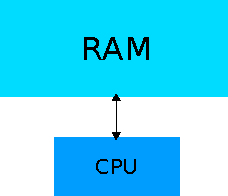
\includegraphics[width=\linewidth]{ram-cpu-simple.pdf}
\caption{Simplistic view of CPU and RAM.} \label{fig:1a}
\end{subfigure}
\hfill
\begin{subfigure}{0.4\textwidth}
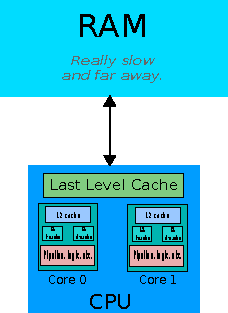
\includegraphics[width=\linewidth]{ram-cpu-complex.pdf}
\caption{More realistic view of CPU and RAM.} \label{fig:1b}
\end{subfigure}
\label{fig:cpu-and-ram}
	\caption[Simplistic versus realistic view of processor and memory.]{View of programming that programmers like to have (a), versus the the more realistic
	and complicated view (b). The cache system is more complicated than will be described here, and the pipeline logic is
	also a significant factor in optimization which will also be glossed over.}
\end{figure}

\subsubsection{Caching}

On modern processor chips, the vast majority of the silicon is used to implement a memory cache. This gives an indication
of how important it is. Think of the cache as a smaller, but much much faster memory that the processor accesses whenever
it would access RAM. If it finds the value in the cache, reading a value can take between 1 and 10's of nanoseconds. However,
if it does not find the value in the cache, it must then perform a read from memory, which can take hundreds of nanoseconds.
For scale, a single instruction often takes less than a nanosecond to do. This means that if a program makes a lot of
memory accesses, the processor will spend a lot of time waiting and not much time calculating.

Earlier in this document, I described a phenomenon which describes how important caching is. Given a 2-D array, there are two
ways to iterate over the whole thing: line-by-line or column-by-column. On my computer, the line-by-line method was five times
faster than the alternative. This has to do with the cache, and specifically, \textit{cache lines}. When reading a value out
of memory for the first time, the processor actually reads many values, something like 64 bytes worth of data. This is a fact
of the design of the hardware, and is partly because if you read a value $x$ from RAM, the processor expects you will want to
access memory that is nearby $x$ in the near future. Thus, if you iterate over an array line-by-line, when you access the
first element of a line you are actually reading in multiple elements of the array into the cache at once. When the processor
then tries to access the second element of the line, it finds that it is already in the cache, making that access much faster
than if it had not been in the cache. If you iterate over the array column-by-column, you read the first element of the line,
which loads several elements from that line into the cache, and then \textit{those values are ignored} and the first element
of the second line is read. This means that when reading the first element of the lines, each time the processor has to fetch
the value from RAM and does not get a chance to make use of the cache. By the time an entire column has been read, the cache
may be full, forcing the processor to remove old values from it. Then, when the program reads the second element of the first line,
that data are no longer in the cache. This is extremely slow.

If possible, try to keep the amount of memory that the program accesses small. Try to organize the access patters such that it is
something that the processor is good at handling (like the iteration direction choice above). I have utilized these methods in my
solver program. An example for keeping memory footprint small was to reuse variables inside the grid that I knew were safe to reuse.
Additionally, I used \texttt{float}s instead of \texttt{double}s wherever possible, as this reduces memory usage as well. Finally,
I made sure to access data in a sequential manner and I ensured that the memory I was accessing was as contiguous as possible.

\subsection{Structure of Arrays}

While I had written code that utilized the x86 SIMD extensions, this was not particularly necessary. Modern compilers are capable
of producing executables which use these instructions themselves, without the help of the programmer. Of course, a skilled programmer
may be able to write a much better version than the compiler can because they have much more context for what the program is doing,
but in general, the compiler can produce a somewhat reasonable output a lot of the time. However, one thing that it cannot do
effectively is reorganize data access patterns into a more CPU friendly manner.

This is the reason why it is, at this point in compiler technology, worth it to restructure performance critical code to help out
the compiler and the processor as much as possible. The structure-of-arrays versus array-of-structures design options are an example
of this. As I described in Section~\ref{sec:opt-mul}, there can be a significant improvement from restructuring to a structure-of-arrays
style of data organization. This is due to, for the most part, the SIMD nature of data processing. The code emitted by the compiler
is likely using SIMD style data accesses, and they are helped tremendously by being able to load a lot of the same value from different
cells at once. Because organizing the data in a SOA method places all of the values that have the same meaning for each cell next to
each other, there is a benefit seen both in the way the code is trying to access the data and in the way the processor is caching it.
Because the simulation uses neighboring cells (half of which are directly adjacent to the current value), organizing the data
in a SOA manner means that it is likely that half of the neighboring cells will be in the same cache-line as the current cell, thus
speeding up their memory accesses drastically.

\subsection{Multi-threading}

Multi-threading a program is a solution to performance problems that is commonly thrown out in a loose way. Multi-threading something is
typically only effective when there are multiple largely independent pieces of work to be done in a system. It does not always improve
performance. This is a situation, like any other performance question, where it is important to measure before and after and determine
if it is worth it.

\subsubsection{Undefined Behavior Land}

One huge problem in multi-threaded programming is data synchronization. Consider a simple example, where there are four threads which
are all sharing a variable named $x$ which initially starts with a value of 4. If all threads execute the code \texttt{x++}, what are
the possible value\textbf{s} of $x$? Ideally, just 8, but that is not the case. The reason is because \texttt{x++} is really three
separate operations: 1) read $x$ into the CPU, 2) increment the value inside the CPU, and 3) write the new value to $x$ in memory.
So what happens if two threads read $x$ at the same time? They both get back 4, and the both increment it internally to 5, and write
back 5, resulting in two increment operations appearing as if only one had happened.

The answer is, $x$ could be 5, 6, 7, or 8, and there is \textit{no way to predict which one}. At least one increment will happen, and
that is all that can be known\footnote{Technically, this is not really true, as this is undefined behavior which is quite literally undefined, and
so your program could do anything from incrementing $x$ to 9 to selling your liver on the black market (though this is admittedly unlikely).}. This is an example of undefined
behavior and is common in multi-threaded programs.

Fortunately, C11 provides a simple solution: declaring variables as \textit{atomic}\footnote{The name referring to small indivisible units, since \textit{atomic operations} are
indivisible (all or nothing).} (for example, \texttt{\_Atomic int x}). If $x$ in
the example above were to be declared this way, then the answer to the above problem is simply ``just 8''. The advantage is that there
is no loss of information when multiple threads operate on a single shared variable. The disadvantage is that this is slower because
it effectively ``locks'' that part of the memory and prevents other operations from occurring until one completes. This is supported
in hardware for integer types, but not floating point types. This makes atomic floating point variables particularly slow because they
need extra locking, and therefore extra memory accesses and CPU time for every access.

This was the problem I ran into when designing the multi-threading in the solver application. There was a shared floating point value
to keep track of how much the simulation had changed after each iteration. This ended up being slower than the single-threaded case.
By minimizing the shared state between threads and limiting the communication of floating point values between threads as much as
possible, there was a huge performance improvement.

\subsubsection{More Threads Means More Data}

An additional concern with multiple threads is that you can run out of cache space more easily. Now, instead of sequentially operating
on some block of data (because sequential data access is fast, so that is what you would do, of course), there are multiple threads
working on different parts of memory at the same time. This means they are fighting over cache space. It is entirely possible for
adding threads to make something \textit{slower}, because of this contention. Again, the key comes down to measuring. It is hard to
know ahead of time what will help and what will not. Multi-threading only makes things worse, since now the program can be run in a
non-deterministic manner: sometimes some threads will be slower, sometimes they will be faster. This makes it even harder to predict,
and more complicated to measure.

\subsection{Branch Reduction}

In programming, any statement in the language which will cause the flow of execution of the code to change based on a condition
is called a branch. This includes if statements, while loops, etc. Many times these cannot be avoided, but there are also
times when the code can be restructured in a way to reduce their number. This can be useful, because branches are often slow.
This is partially because of caching (instructions for the CPU are cached as well as data, so if it suddenly jumps far away due
to a branch, it has to load instructions from memory, which is slower). The real reason that branches are slow has to do with
pipelining in the CPU, which I will not go into here. The summary is that reducing branches is good, and organizing the required
branches in a simple way will probably be good enough for the processor to optimize them reasonably well.

\subsection{Concluding Remarks}

The most important idea when optimizing is to keep in mind that you may be wrong, so measure everything to ensure that the optimization
is actually an optimization. Secondly, a highly optimized but slow algorithm will still be slow for large enough inputs. Fast processors
do not beat order notation, and searching a hash table for a value ($O(1)$) is \textit{extremely likely} to be faster than looking it up
in an array ($O(n)$). Thirdly, make sure that there is no hidden cost in using a data structure, avoid repeated work that does not need to be repeated,
and be aware of some basic reasonably fast algorithms (sorting, for example). Fourth, use a programming language which compiles to direct processor
instructions (C, C++, among others), and use the optimization options for the language. Fifth, organize the program's data so that accessing it is
typically sequential, and try to design the layout of data such that it is easy for the compiler and the processor to optimize. Sixth, multi-threading
can help, but it can also be tricky to get right. Finally, work on reducing memory footprint, branches, code complexity, and complicated slow
math if possible.

That said, programs should be written for correctness and clarity first, even if this means sacrificing some performance early on. However,
there is a limit to this. Faster algorithms should be used, and we should try hard not miss Donald Knuth's 3\%, as long as we remember to measure
what we have done.
